% !TeX program = xelatex
% 大学生创新创业训练计划 项目中期检查表（心安动识 / 基于多传感器融合的BFRBs智能检测系统研究）
% 编译：xelatex 中期检验报告.tex
\documentclass[12pt, a4paper]{ctexart}

\usepackage{geometry}
\geometry{margin=2.2cm, top=2.4cm, bottom=2.4cm}
\usepackage{graphicx}
\usepackage{booktabs}
\usepackage{array}
\usepackage{xcolor}
\usepackage{enumitem}
\usepackage{float}
\usepackage{caption}
\captionsetup{font=small, labelsep=quad}

\definecolor{warmpink}{RGB}{174, 105, 82}
\newcolumntype{L}[1]{>{\raggedright\arraybackslash}p{#1}}
\setlist{nosep, leftmargin=1.6em}
\linespread{1.35}

\begin{document}

% ==================== 表头 ====================
\begin{center}
{\Large\bfseries 大学生创新创业训练计划\par}
\vspace{0.3em}
{\LARGE\bfseries 项目中期检查表\par}
\end{center}

\vspace{1em}
\begin{center}
\renewcommand{\arraystretch}{1.6}
\begin{tabular}{|L{3.2cm}|L{5.6cm}|L{3.2cm}|L{4.2cm}|}
\hline
\textbf{项目编号} & S202610511201 & \textbf{成果形式} & 其他研究报告 \\ \hline
\textbf{项目名称} & \multicolumn{3}{L{10.6cm}|}{基于多传感器融合的身体聚焦重复行为（BFRBs）智能检测系统研究（心安动识 MindEase）} \\ \hline
\textbf{项目成员} & 杨博文、吴裕熙、苏钰柔 & \textbf{指导老师} & 吴彦文 \\ \hline
\textbf{项目时间} & \multicolumn{3}{l|}{2026 年} \\ \hline
\end{tabular}
\end{center}

\vspace{0.8em}

% ==================== 一、项目进展情况 ====================
\section*{一、项目进展情况}

\begin{center}
\renewcommand{\arraystretch}{1.4}
\begin{tabular}{|L{7.4cm}|L{7.4cm}|}
\hline
\centering\textbf{预期研究成果} & \centering\textbf{实际研究成果} \tabularnewline \hline
$\boxtimes$ 其他：\newline
"心安动识"情绪识别与心灵疗愈 Web 平台（可运行系统）；\newline
BFRBs 智能检测模型与研究报告；\newline
学术论文 1 篇（已发表，版面费已报销）。 &
$\boxtimes$ 其他：\newline
平台三端（Vue 前端 / Spring Boot 后端 / Flask YOLO 推理）已落地并跑通全部核心功能；\newline
五类 BFRBs 行为检测模型 \texttt{bfrb\_behavior.pt} 训练完成（同源验证集 mAP50 = 0.744）；\newline
皮肤损伤痕迹检测模型 \texttt{bfrb\_wound.pt}（mAP50 = 0.519）；\newline
自建数据管线与数据集（FaceTouch 公开数据 + 自录视频，合并训练集 1594 张）；\newline
双视角预诊报告、「心有灵犀」医患联动模块、心灵 SPA 专属疗愈地图均已上线；\newline
后端 12 项自动化测试全部通过，核心流程经浏览器端到端走查验证。 \tabularnewline \hline
\end{tabular}
\end{center}

% ==================== 二、能否按计划进行 ====================
\section*{二、项目是否能按计划进行，是否能按时结题（字数小于1000）}

项目整体按计划推进，预计能够按时结题。

技术主线方面，"视觉多通道检测"的核心难点——BFRBs 躯体行为识别模型——已完成从
方案调研、数据采集、自动伪标注管线开发到模型首版训练的完整闭环。面对公开渠道无
BFRBs 行为标注数据集的客观约束，团队改用"手脸检测几何规则自动打标 + 人工抽验"的
低成本数据管线，将 FaceTouch 公开数据集（9337 张）与团队自录动作视频（10 段、
覆盖全部五类行为）合并训练，首版模型同源验证集 mAP50 达 0.744，验证了技术路线的
可行性，为后续迭代打下了坚实基础。

平台主线方面，立项时规划的情绪识别、觉察记录、温柔对话等基础功能均已实现；
中期阶段进一步完成了三项计划内深化：预诊报告双视角输出（使用者收到无医学术语的
书信式关怀信，专业人员看到客观报告与安全关注标注）、「心有灵犀」医患联动模块
（双端认证 + 模拟审核流 + 站内书信式对话）、心灵 SPA 疗愈地图接入真实高德地图 API。
学术论文已发表，完成预期的成果形式要求。

进度偏差主要出现在数据积累环节：自录数据目前为单人单场景，跨人群泛化能力
有待提升，已列入下阶段首要任务，不影响总体结题目标。经费使用与硬件准备
（STM32 开发板用于腕戴传感器通道原型）均按计划执行。

综上，项目进度符合预期，团队有信心按计划完成结题。

% ==================== 三、研究阶段成果概述 ====================
\section*{三、研究阶段成果概述（字数小于1000）}

\textbf{1. BFRBs 行为检测专属模型。}自研"视频抽帧 $\rightarrow$ 手脸检测自动伪标注
$\rightarrow$ 数据集合并 $\rightarrow$ 微调训练"全流程工具链，训练出五类行为直检模型
（咬指甲 / 抠皮肤揉眼 / 拔头发抓头皮 / 摸脸 / 手部自然状态），同源验证集
P = 0.731、R = 0.693、mAP50 = 0.744；分类别 mAP50：咬指甲 0.871、抠皮肤揉眼 0.796、
拔头发 0.949。模型已接入推理服务，支持权重热切换，实测可输出行为类别、置信度与
温柔觉察文案。另有皮肤损伤痕迹检测模型作为行为后果辅助通道（mAP50 = 0.519）。

\textbf{2. 双视角预诊报告。}同一份结构化检测数据输出两种形态：使用者视角为书信式
关怀信（AI 生成 + 17 个医学禁词拦截 + 本地温柔模板兜底），专业人员视角为客观预诊
报告并叠加规则式安全关注标注（持续愤怒主导、高频重复行为、自述危险关键词三档），
两者均支持导出 PDF。

\textbf{3. 「心有灵犀」医患联动模块。}实现双端认证体系（心灵SPA师资格认证 /
使用者实名认证，身份证仅存掩码，模拟审核流由管理员通过）与站内书信式对话；
心灵SPA师可查看求助者历史觉察记录并跳转客观预诊参考，形成"线上预诊、
必要时转线下"的流程雏形。

\textbf{4. 心灵 SPA 专属疗愈地图。}接入真实高德地图 API，IP 定位 + 浏览器精确定位，
检索附近 5 公里真实机构（心理咨询/心理门诊/冥想瑜伽/公园绿道/书店茶饮），
机构详情弹窗含真实电话与地址，支持自由缩放。

\textbf{5. 工程质量。}后端 12 项自动化测试全部通过，前端构建通过，
核心流程（注册 $\rightarrow$ 认证 $\rightarrow$ 审核 $\rightarrow$ 倾诉
$\rightarrow$ 双向对话 $\rightarrow$ 查看报告）经真实浏览器端到端走查验证。
系统实测截图见附件。

% ==================== 四、经费使用情况 ====================
\section*{四、经费使用情况和下阶段经费安排计划（字数小于1000）}

本项目经费 5000 元，已基本使用完毕，支出明细如下：

\begin{center}
\renewcommand{\arraystretch}{1.35}
\begin{tabular}{L{4.6cm} r L{7.2cm}}
\toprule
\textbf{支出项} & \textbf{金额（元）} & \textbf{用途说明} \\
\midrule
论文版面费 & 3000 & 阶段性研究成果学术论文发表 \\
STM32 集成开发板（2 块） & 1600 & 腕戴传感器通道硬件原型（多传感器融合扩展） \\
AI 模型订阅 & 200 & 大模型 API 调用（关怀书信生成、陪伴对话） \\
\midrule
\textbf{合计} & \textbf{4800} & 结余 200 元 \\
\bottomrule
\end{tabular}
\end{center}

各项支出均与项目研究内容直接相关，报销流程合规：论文版面费对应成果形式中的
学术成果产出；开发板用于下阶段腕戴传感器采集原型搭建；AI 模型订阅支撑平台
智能文案能力的开发与测试。

下阶段经费安排（以结余及后续追加为准）：（1）传感器原型耗材与配件
（腕带、电池、外壳等）；（2）云服务器短期租用，用于平台公网试运行与
小规模用户体验测试；（3）数据采集中向志愿录制同学支付的少量激励费用；
（4）如有剩余，用于结题材料印制与展示物料。

% ==================== 五、存在问题及解决方法 ====================
\section*{五、存在问题及解决方法（字数小于1000）}

\textbf{1. 伪标注数据存在噪声。}自动标注管线会将部分过渡帧（手在空中尚未接触脸部）
误标为行为类。解决方法：收紧接触判定阈值后重新标注，结合 Roboflow 在线修标工具
人工抽验修正，逐步提高标签质量。

\textbf{2. 模型跨人群泛化能力不足。}自录数据目前为单人单场景，模型在陌生人群、
低清图像上的指标明显低于同源验证集（跨域 mAP50 约 0.212）。解决方法：下阶段
组织多位同学在不同光线、角度、着装下补录动作视频，并混合公开数据训练，
逐步缩小域差。

\textbf{3. 认证体系为模拟审核流。}当前医师资格与实名认证未接入权威核验渠道，
仅做形式校验与人工审核占位。解决方法：保留审核状态与数据字段设计，待与学校
心理中心或合作医院对接后接入真实核验流程。

\textbf{4. 医患权限尚未细化。}报告双视角目前是视角切换而非权限门控，医生身份
访问控制需在真实合作场景中完善。解决方法：在「心有灵犀」模块中已实现基于身份
认证状态的功能门禁，下一步将补充基于角色的访问控制与操作审计。

% ==================== 六、下阶段工作计划 ====================
\section*{六、下阶段工作计划（字数小于1000）}

\textbf{1. 数据扩充与模型迭代（第 1--5 周）。}组织 3--5 名同学在不同光线、角度、
着装条件下补录五类行为视频；用现有伪标注管线自动打标并人工修标；
复训行为模型，目标同源 mAP50 $\geq$ 0.85，显著缩小跨域差距。

\textbf{2. 医院实地调研与合作洽谈（第 3--8 周）。}赴校医院及武汉本地医院
心理门诊实地调研，洽谈「心有灵犀」模块的线上试运营合作，争取真实医生入驻，
并据此完善角色权限与报告流转流程。

\textbf{3. 腕戴传感器通道原型（第 5--10 周）。}基于已购置的 STM32 开发板搭建
腕戴采集原型，采集 IMU 时序数据，参考 Kaggle CMI 公开数据集的方法训练手势
识别模型，与视觉通道形成多传感器融合验证闭环。

\textbf{4. 平台部署试运行（第 8--12 周）。}前端打包由 Nginx 托管，后端常驻运行，
推理服务独立部署，完成腾讯云上线与小规模试用，收集反馈并优化，
整理结题材料与研究报告。

% ==================== 签字 ====================
\vspace{2em}
\noindent 项目负责人签字：\raisebox{-0.9cm}{\includegraphics[height=2.1cm]{midterm-assets/sign-leader.jpg}}\hfill 2026 年 10 月 04 日

% ==================== 七、附件 ====================
\clearpage
\section*{七、其他（附件）：系统实测截图}

\begin{figure}[H]
  \centering
  
\includegraphics[width=0.88\textwidth]{midterm-assets/homepage.png}
  \caption{平台首页（温柔治愈风格）}
\end{figure}

\begin{figure}[H]
  \centering
  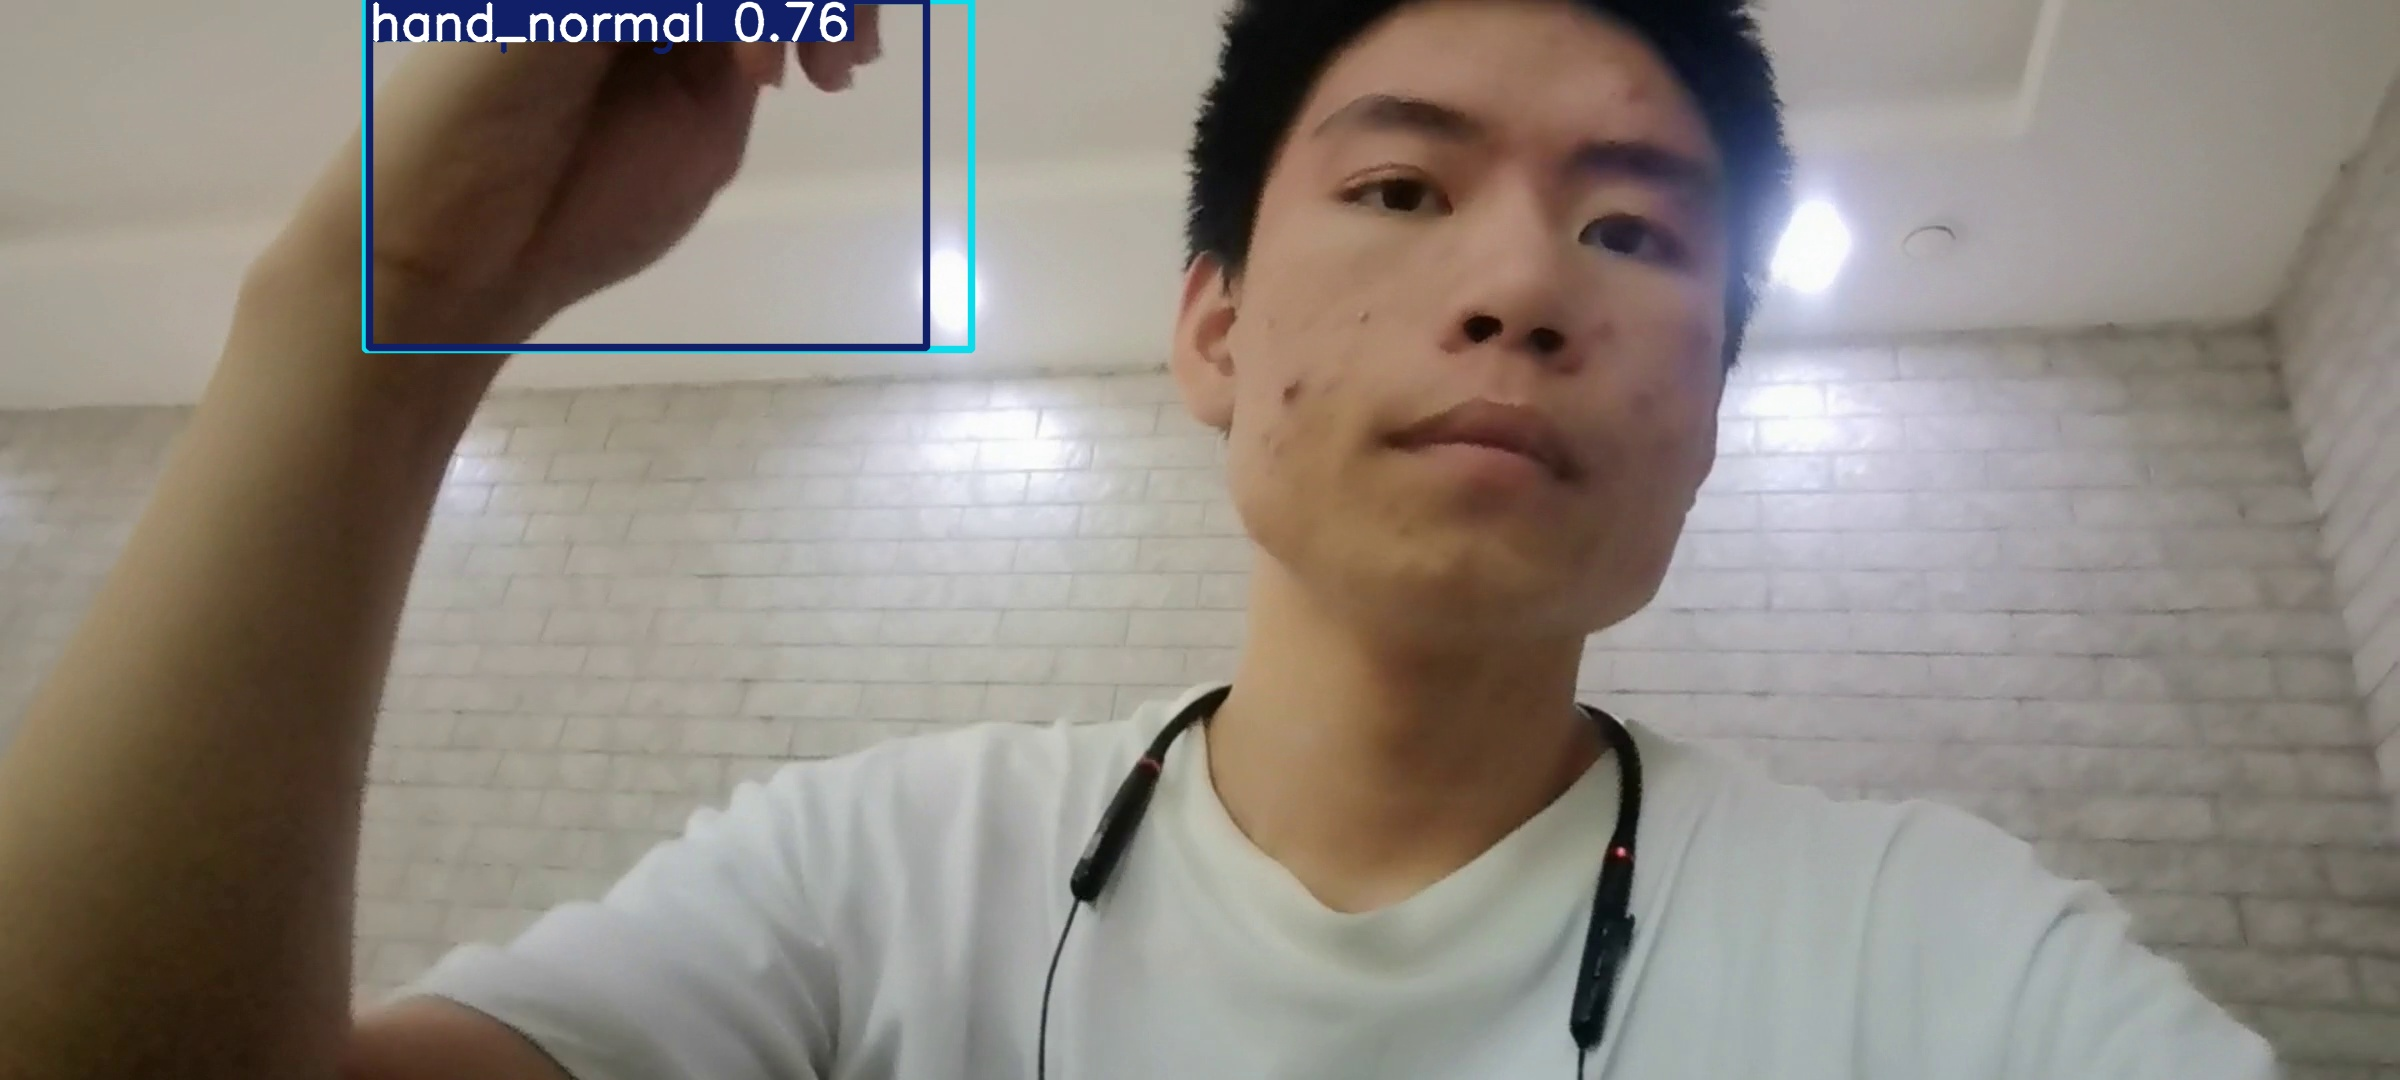
\includegraphics[width=0.6\textwidth]{midterm-assets/bfrb-inference.jpg}
  \caption{BFRBs 行为模型推理实测（检出抠皮肤揉眼类线索与手部自然状态）}
\end{figure}

\begin{figure}[H]
  \centering
  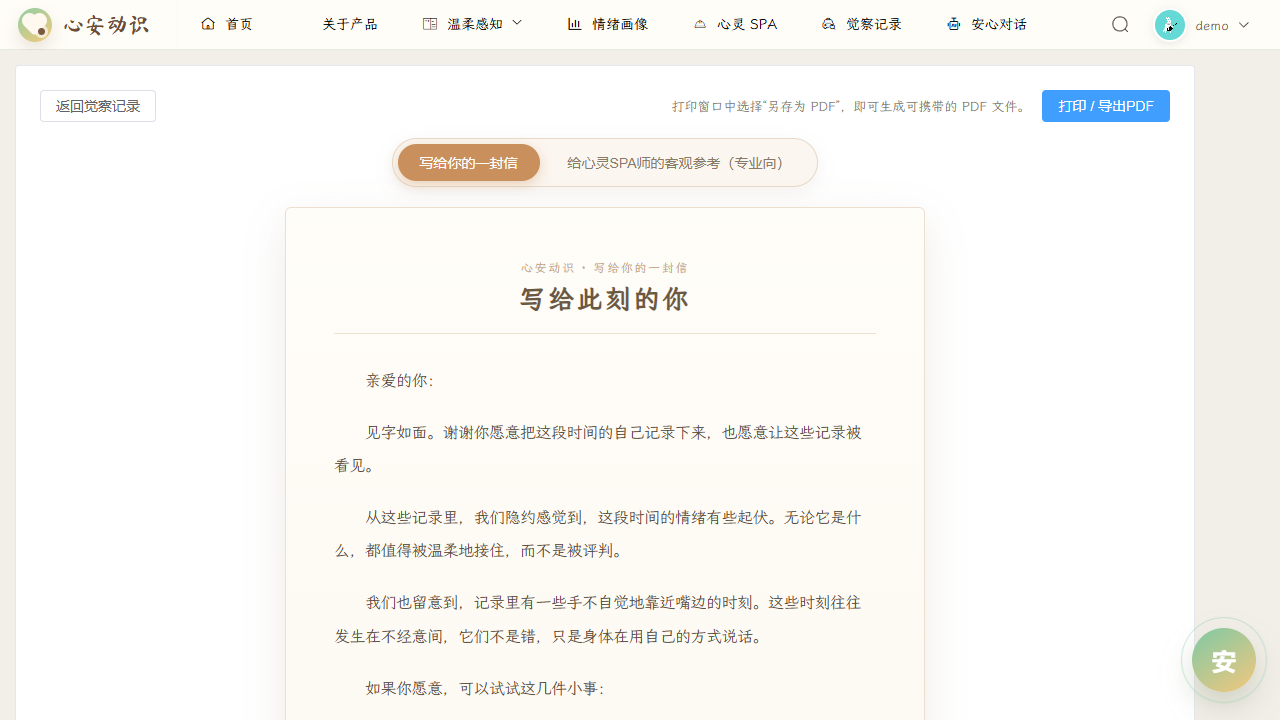
\includegraphics[width=0.88\textwidth]{midterm-assets/care-letter.png}
  \caption{双视角预诊报告·使用者视角（书信式关怀信，无医学术语）}
\end{figure}

\begin{figure}[H]
  \centering
  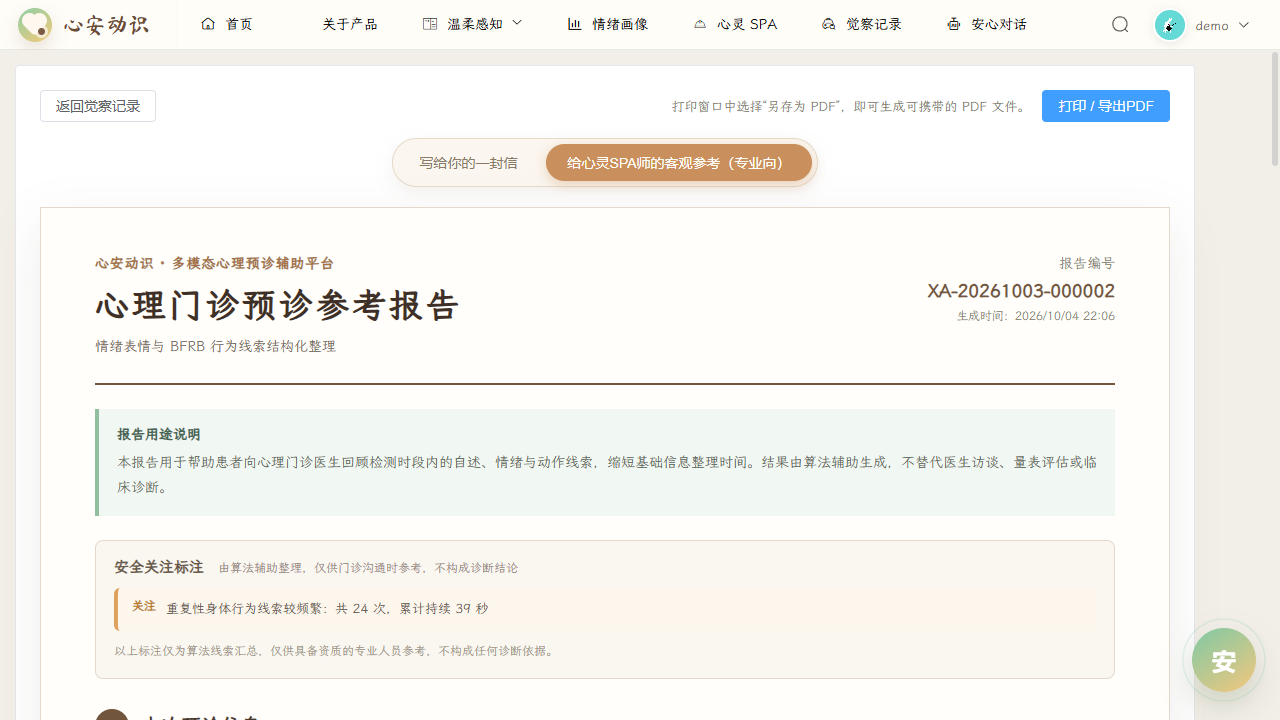
\includegraphics[width=0.88\textwidth]{midterm-assets/clinician-view.png}
  \caption{双视角预诊报告·心灵SPA师视角（客观报告 + 安全关注标注）}
\end{figure}

\begin{figure}[H]
  \centering
  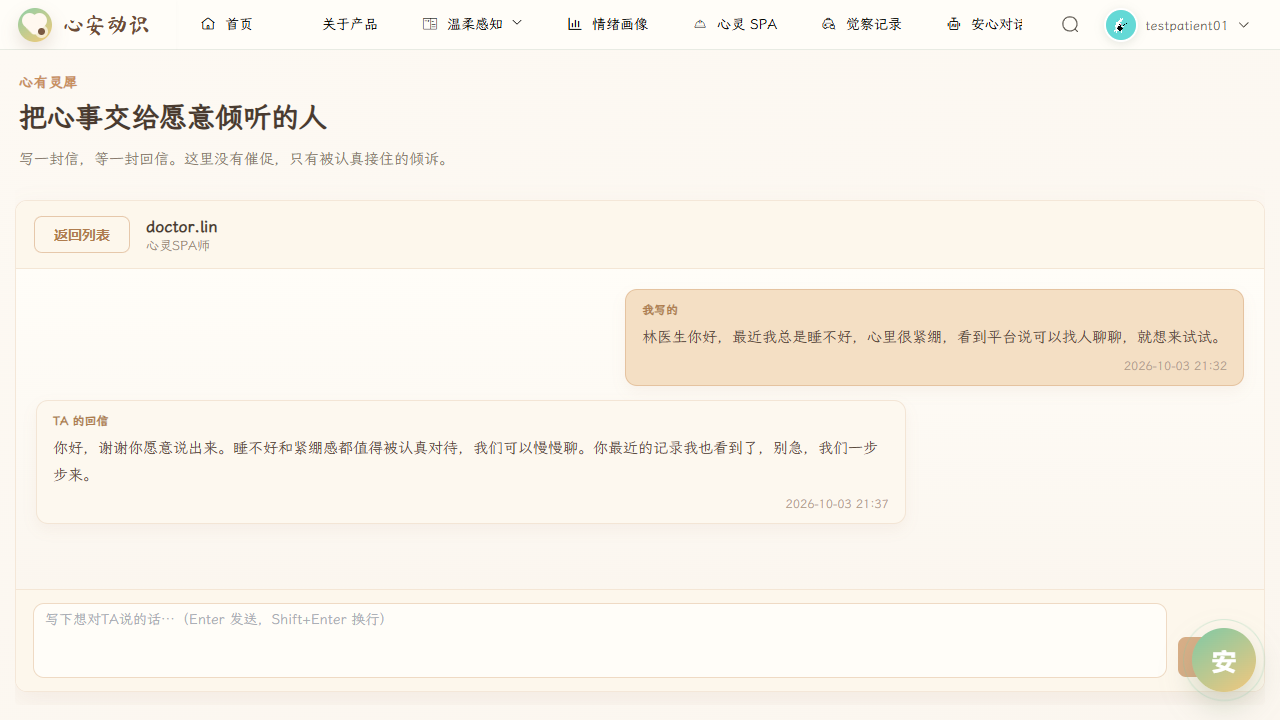
\includegraphics[width=0.88\textwidth]{midterm-assets/spa-conversation.png}
  \caption{「心有灵犀」书信式医患对话}
\end{figure}

\begin{figure}[H]
  \centering
  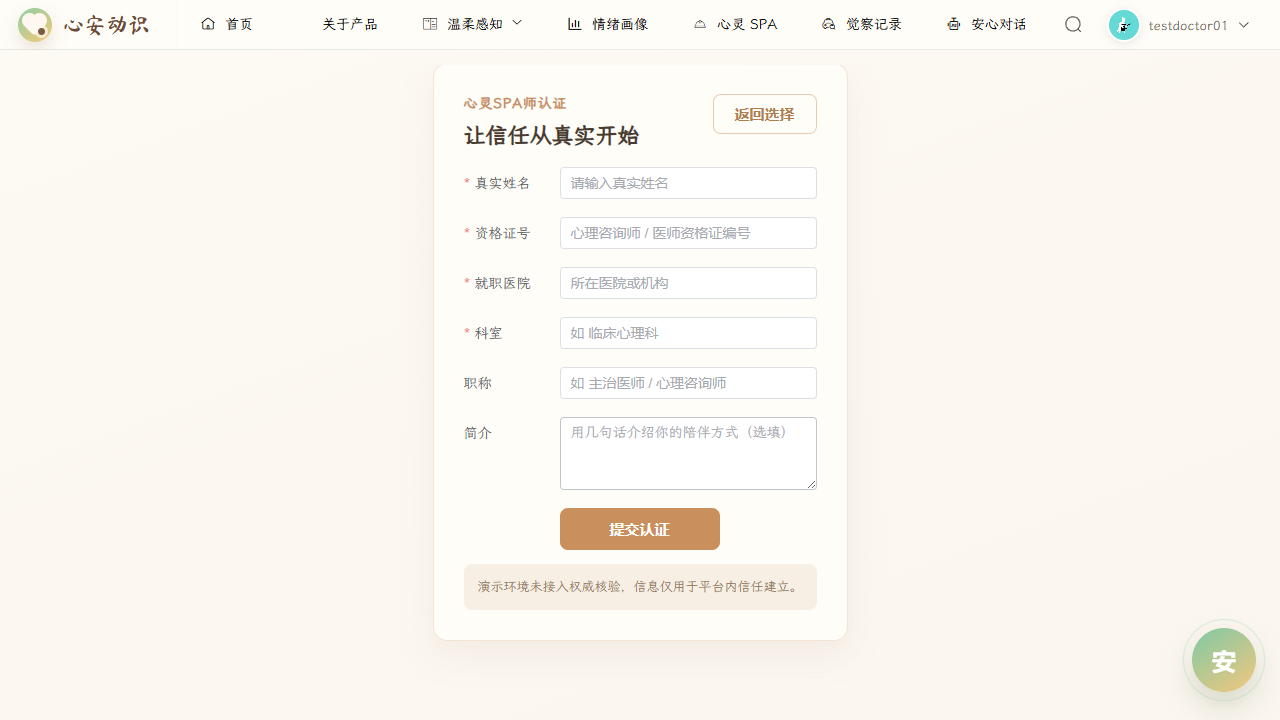
\includegraphics[width=0.72\textwidth]{midterm-assets/identity-cert.png}
  \caption{心灵SPA师认证表单（模拟审核流）}
\end{figure}

\begin{figure}[H]
  \centering
  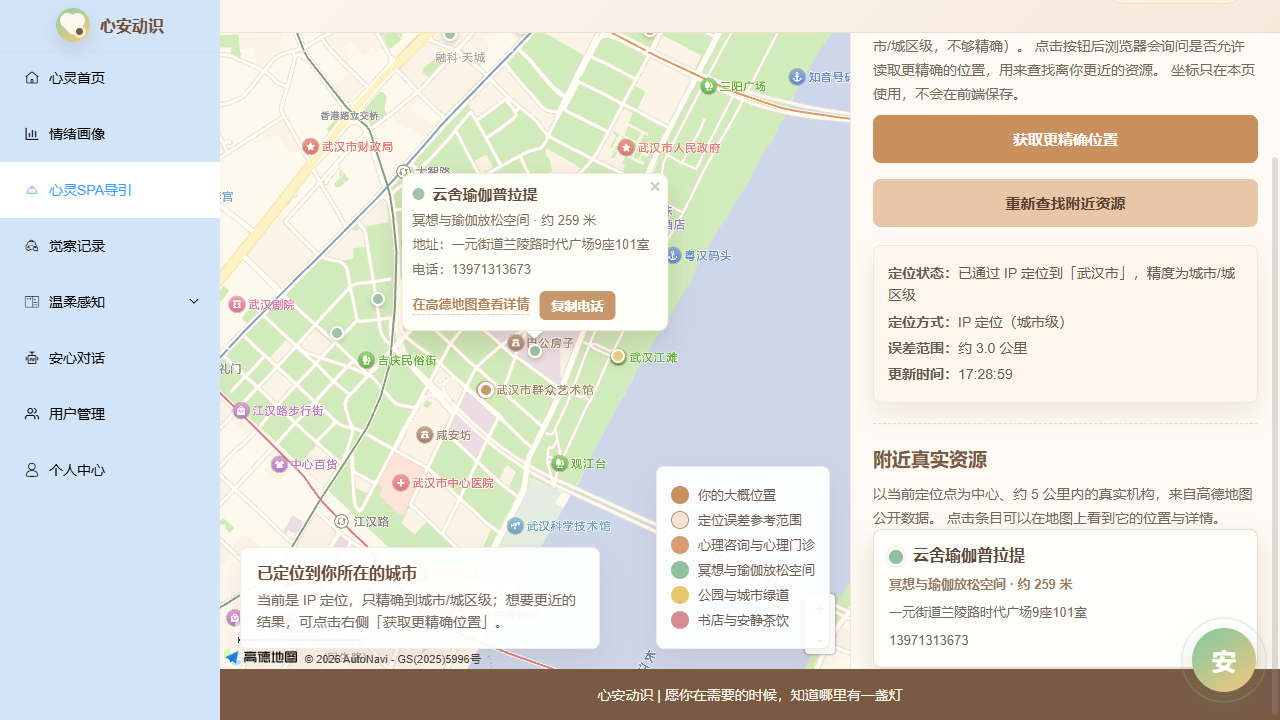
\includegraphics[width=0.88\textwidth]{midterm-assets/healing-map.png}
  \caption{心灵 SPA 专属疗愈地图（真实高德数据 + 机构详情弹窗）}
\end{figure}

% ==================== 八/九/十、意见栏 ====================
\clearpage
\section*{八、指导教师意见（字数小于200字）}

\vspace{1em}
\noindent 同意。

\vspace{3.5cm}

\noindent 签字：\raisebox{-0.55cm}{\includegraphics[height=1.5cm]{midterm-assets/sign-advisor.jpg}}\hfill 2026 年 10 月 04 日

\vspace{1.5em}
\section*{九、院系意见}

\vspace{4.5cm}

\noindent 签章：\rule{4cm}{0.4pt}\hfill \rule{2cm}{0.4pt} 年 \rule{1.2cm}{0.4pt} 月 \rule{1.2cm}{0.4pt} 日

\vspace{1.5em}
\section*{十、学校意见}

\vspace{4.5cm}

\noindent \hfill \rule{2cm}{0.4pt} 年 \rule{1.2cm}{0.4pt} 月 \rule{1.2cm}{0.4pt} 日

\end{document}
